\documentclass[a4paper,12pt]{article} 
% Paquetes......................................................................
\usepackage{amsmath, amssymb, amsfonts, latexsym}
\usepackage[utf8]{inputenc}
\usepackage[T1]{fontenc}
\usepackage{palatino}
\usepackage[full]{textcomp}
\usepackage{hyperref}
\usepackage{eurosym}
\usepackage[makeroom]{cancel}
\usepackage{array}
\usepackage{pdfpages}
\usepackage{float} % para que las figuras no floten
\usepackage{subcaption}

\textheight = 24 cm
\textwidth = 17 cm

\renewcommand{\arraystretch}{1.25}
\renewcommand{\contentsname}{Contenidos}


% INICIO DEL DOCUMENTO --------------------------------------------------------
\begin{document}
	
	\setlength{\parindent}{0.5cm}
	\setlength{\voffset}{-2cm}
	\setlength{\hoffset}{-2cm}
	
	\begin{center}
		\begin{LARGE}
			\textbf{Práctica Grupo 3}
		\end{LARGE}
		\begin{Large}
			\\ \medskip \text{Luis Couto Seller, Irene Marbán, Aída Muñoz Monjas}
		\end{Large}
		\rule{14cm}{0.5mm}
	\end{center}
	
	
	\tableofcontents
	
\newpage
	\section*{Ejercicio 1}
	\addcontentsline{toc}{section}{Ejercicio 1}
	\textbf{Generación de números y variables aleatorias.} Describir el método \textit{Monty Phyton} para la distribución normal y compararlo con otros métodos para la
generación de valores de la normal.
	
	El objetivo del método Monty Python es lograr generar números aleatorios cuya frecuencia se aproxime a aquella de una distribución normal. Para ello, emplea la similitud entre la expresión de la función de densidad de la distribución normal y una sigmoide decreciente, así como se aprovecha del bajo coste computacional de la generación de números aleatorios en un rectángulo.
	$$ N(0,1) \sim f(x) = \dfrac{1}{\sqrt{2\pi}} \cdot e^{-x^2/2} $$
	
	Tomando $x>0$, se traza un rectángulo de base $b$ y altura $1/b$ sobre la sigmoide. Con un giro de $\pi$ radianes y un desplazamiento sobre la región exterior al rectángulo se pretende representar la mayor superficie posible de la sigmoide en el interior del rectángulo de área $1$. En las imágenes siguientes, podemos observar el procedimiento descrito tomando un $b=2.29$
	
	\begin{figure}[H]
		\begin{subfigure}{.5\textwidth}
			\centering
			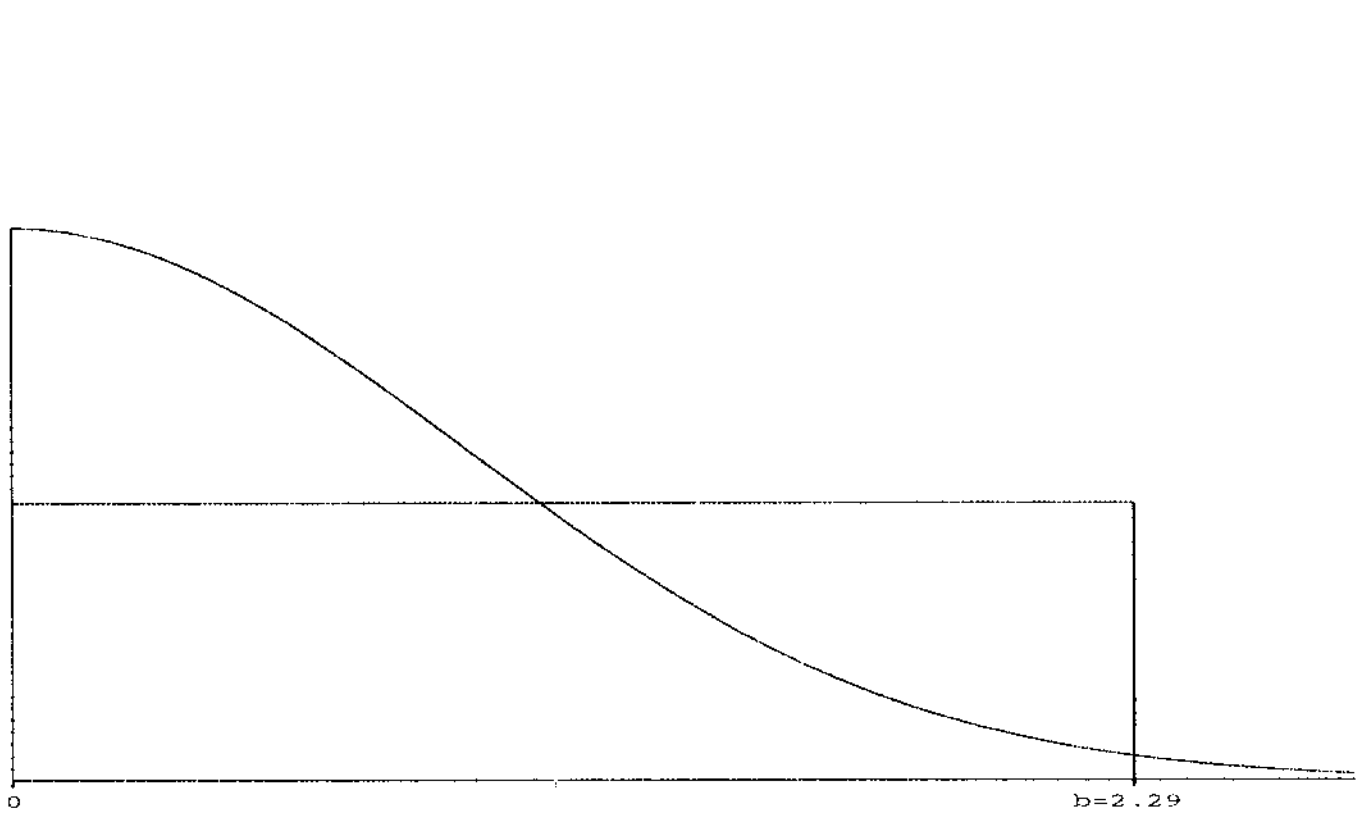
\includegraphics[width=\textwidth]{include/sigmoid_w_square.png}
			\caption{Sigmoide con el rectángulo de base $b$. \cite{monty-python}}
		\end{subfigure}
		\begin{subfigure}{.5\textwidth}
			\centering
			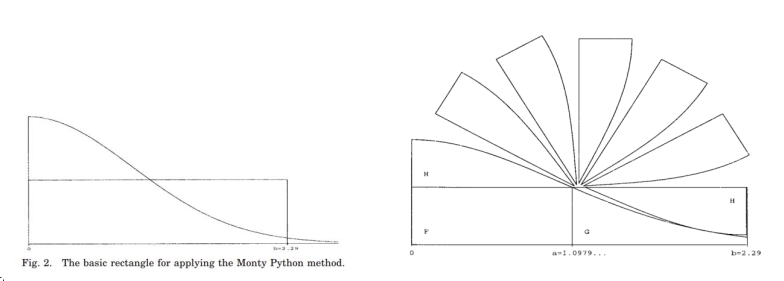
\includegraphics[width=\textwidth]{include/rotating_sigmoid.png}
			\caption{Giro y desplazamiento gráficamente. \cite{monty-python}}
		\end{subfigure}
	\end{figure}
	
	Una vez descrito el área bajo la función de densidad en el interior del rectángulo, todo número aleatorio generado en ese rectángulo pertenecerá a las regiones $F$, $G$, $H$ o a la región comprendida entre $G$ y $H$ correspondiente a la cola de la sigmoide. La probabilidad de obtener un número en la cola es de un $0.022$ \cite{monty-python}.
	
	Entonces, siendo $(x,y)$ el valor aleatorio generado y $(x',y')$ su valor correspondiente en la sigmoide, se tiene
	$$
	(x',y') = 
	\begin{cases}
		(x,y) \quad \text{si} \quad x\in F \text{ ó } G \\
		(b-x,2/b-y) \quad \text{si} \quad x \in H
	\end{cases}
	$$  
	
	Si el valor aleatorio generado no pertenece a $F$, $G$ ó $H$, pertenecerá a la cola de la distribución, por lo que basta con devolver una variante de la cola normal mediante el método de Marsaglia o el método de la cola general de Marsaglia y Tsang.\\
		
	La elección del valor de $b$ no es crítica, pero elegir un valor de $b$ demasiado grande implica que habrá solapamiento al realizar el giro y desplazamiento descrito, mientras que si el valor de $b$ es demasiado pequeño, será necesario realizar frecuentemente el método para hallar los valores de la cola.
	En caso de utilizar el método anterior para "ajustar" la sigmoide al rectángulo, la elección de $b=2.29$ es prácticamente la máxima posible \cite{monty-python}. \\
		
	En lugar de una rotación y un desplazamiento de la región exterior al rectángulo, "estirar" la región $H$ permite un ajuste mejor, manteniendo constante el área de la sigmoide, y por tanto siendo este un método más complejo pero más eficiente para realizar dicha aproximación. 
	
	Definiendo el factor de estiramiento $s$ y la función de densidad de la región $H$ $f_H(x)$ como 
	$$s=\dfrac{a}{b-a} \hspace{1.5cm} f_H(x)=f(x)-\dfrac{1}{b} \hspace{2mm} \text{con} \hspace{2mm} 0<x<a $$
	
	Por lo tanto, la región $H$ girada y estirada tiene una función de densidad
	$$ f_{H'}(x) = \dfrac{1}{b} - s  \left[ f(s (b-x) ) -\dfrac{1}{b} \right] $$ 
	La siguiente figura representa gráficamente las transformaciones matemáticas descritas compuestas con la rotación aplicada a la sección $H$. 
	
	\begin{figure}[H]
		\centering
		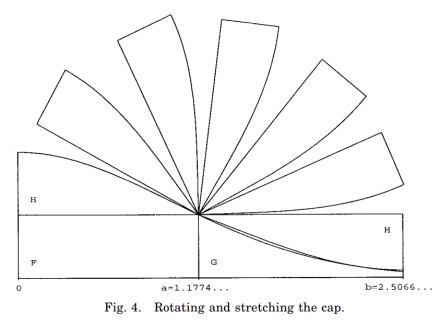
\includegraphics[width=0.6\textwidth]{include/stretching_sigmoid.png}
		\caption{Descripción gráfica del estiramiento descrito. \cite{monty-python}}
	\end{figure}
	
	Para este segundo caso, la elección habitual para el valor de $b$ es $b= \sqrt{2\pi}$. Esta elección no es crítica, cualquier valor entre $2.506$ y $2.5074$ es válido \cite{monty-python}, pero el par $b=\sqrt{2\pi}$, $a = \sqrt{\ln 4}$ son opciones fácilmente identificables con una precisión ilimitada.
	
	
\newpage
	\section*{Ejercicio 2}
	\addcontentsline{toc}{section}{Ejercicio 2}
	\textbf{Simulación de sucesos discretos y optimización.} Consideremos un almacén de dos productos cuyos precios de venta al público
 son de $2.5$ y $3.5$ euros la unidad, respectivamente. La llegada de clientes al
almacén se distribuye según un proceso de Poisson de parámetro $\lambda = 1.5$ clientes
por hora y la cantidad de productos demandados por cada uno de ellos tiene la
siguiente distribución:
	
	\begin{table}[H]
		\centering
		\begin{tabular}{|l||c|c|c|c|}
			\hline
			Demanda    & 1 unidad & 2 unidades & 3 unidades & 4 unidades \\ \hline \hline
			Producto 1 & 0.3      & 0.4        & 0.2        & 0.1        \\ \hline
			Producto 2 & 0.2      & 0.2        & 0.4        & 0.2        \\ \hline
		\end{tabular}
	\end{table}

	Para satisfacer la demanda de sus clientes el dueño del almacén mantiene un
 stock de productos. La política de pedidos al distribuidor es periódica, es decir
 todos los viernes a primera hora realiza un pedido en el que tomando como
referencia el nivel de inventario de los productos en ese Para satisfacer la demanda de sus clientes el dueño del almacén mantiene un
 stock de productos. La política de pedidos al distribuidor es periódica, es decir
todos los viernes a primera hora realiza un pedido en el que tomando como
referencia el nivel de inventario de los productos en ese momento, se solicitan
las unidades necesarias para que el nivel del inventario de cada producto llegue
a $1000$ y $1500$ unidades, respectivamente en cada producto.

	
	Asociado a cada pedido que realizamos al proveedor existe un coste fijo (coste
de preparación) de $100$ euros, independientemente de las unidades
demandadas. Adicionalmente, el coste por unidad incluida en el pedido depende de la cantidad solicitada habiendo descuentos por cantidad. Si el número de
unidades demandadas del primer producto es menor o igual a $600$ el precio es
de $1$ euro la unidad, mientras que si se piden más de $600$ el precio desciende a
$75$ céntimos. Para el segundo producto, si el número de unidades demandadas
es menor que $800$ el precio es de $1.5$ euros la unidad, mientras que si se piden
más de $800$ el precio desciende a $1.25$ euros.
	
	El tiempo que tarda en ser servido el pedido por los proveedores (tiempo líder),
sigue una distribución normal de media 48 horas y desviación típica $3.5$,
pagándose en ese momento.
	
	Se ha llegado a un acuerdo con el proveedor de forma que, tomando como
referencia las $48$ horas que tarda en media un pedido en ser servido, si el pedido
llega con $3$ horas de retraso en la entrega del mismo se realiza un descuento del $0.03\%$ del valor del pedido, encareciéndose en la misma cantidad en el caso de
que el pedido llegue con al menos $3$ horas de adelanto.

	
	El dueño del almacén debe pagar $0.0002$ euros por unidad del producto y
unidad de tiempo, asociado al almacenamiento físico de los productos (alquiler
del local, refrigeración...).
En el caso de que al llegar un cliente éste solicite una cantidad mayor que la que
hay en inventario, se le sirve lo que queda, perdiendo la venta restante.
	
	\begin{enumerate}
		\item[a)] Simular el comportamiento de almacén durante un periodo de tiempo de $5$
meses para estimar el beneficio esperado, la proporción de clientes cuya
demanda se satisface completamente y el porcentaje de tiempo que el nivel del
inventario permanece a cero. Para ello, supondremos que el nivel del inventario
inicial es de $70$ unidades de ambos productos.
		\item[b)] Representar gráficamente la evolución del nivel del inventario durante los $5$
meses y durante los $5$ primeros días.
		\item[c)] Mediante el uso de la metaheurística recocido simulado identificar cuál será la
política de pedidos óptima, es decir, identificar cada cuánto tiempo se deberían
realizar los pedidos y el valor de referencia del inventario para identificar el
número de unidades a solicitar en la política de pedidos periódica.
	\end{enumerate}

	\textbf{Nota.} El almacén permanece abierto las $24$ horas al día de lunes a domingo. El
proveedor y la empresa transportista (que sirve los pedidos) también trabajan
las $24$ horas, no cerrando en ningún momento.
	
	
	
\newpage
	\section*{Bibliografía}
	\addcontentsline{toc}{section}{Bibliografía}
	\bibliography{include/references}
	\bibliographystyle{IEEEtran}
	
\end{document}